\documentclass[a4paper,11pt]{article}
\usepackage[T1]{fontenc} % if needed
\usepackage{amsmath}
\usepackage{amssymb}
\usepackage{graphicx,float,caption,tikz,subcaption,pgfplots}
\usepackage{color}
\usepackage{xcolor}

\begin{document}

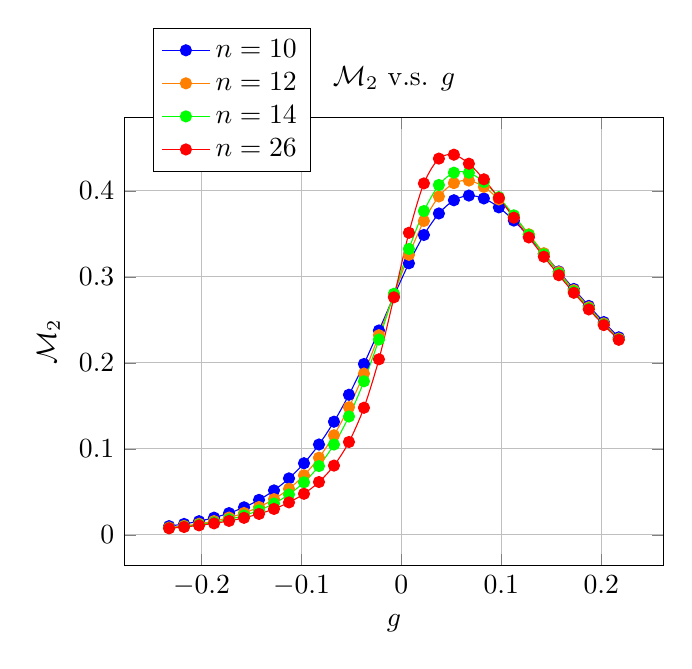
\begin{tikzpicture}
    \begin{axis}[
        xlabel={$g$}, % Set the label for the x-axis
        ylabel={$\mathcal{M}_2$}, % Set the label for the y-axis
        title={$\mathcal{M}_2$ v.s. $g$ },
        tick align=inside, % Aligns the ticks to the outside
        legend style={at={(0.2,1.2)},anchor=north}, % Position the legend below the plot
        grid={both}
    ]
    \addplot[
        color=blue,
        mark=*, % This specifies the type of mark at each data point
        smooth % This option smoothes the line
    ] coordinates {
        (-0.2324768366025517, 0.010179027166607601)
         (-0.2174768366025518, 0.012700677518416869)
         (-0.20247683660255178, 0.015914929866794172)
         (-0.18747683660255177, 0.020024212927263287)
         (-0.17247683660255175, 0.02528791586737733)
         (-0.15747683660255174, 0.032034550069390655)
         (-0.14247683660255173, 0.04067294569286466)
         (-0.1274768366025517, 0.05169871325524065)
         (-0.11247683660255181, 0.06568911429733332)
         (-0.09747683660255169, 0.08327519508063366)
         (-0.08247683660255178, 0.10507537532282413)
         (-0.06747683660255177, 0.13157250926463754)
         (-0.05247683660255176, 0.16292287590693638)
         (-0.037476836602551744, 0.19870953869174304)
         (-0.02247683660255173, 0.2376998361713844)
         (-0.0074768366025518285, 0.27772582130124907)
         (0.007523163397448296, 0.31583345964325205)
         (0.022523163397448198, 0.348777714878471)
         (0.03752316339744832, 0.37375895572844275)
         (0.052523163397448225, 0.3891051689553718)
         (0.06752316339744824, 0.3945830900350399)
         (0.08252316339744825, 0.39122799220737287)
         (0.09752316339744815, 0.38084991622703784)
         (0.11252316339744828, 0.36548868544182306)
         (0.12752316339744818, 0.3470148330281814)
         (0.1425231633974483, 0.32693104318822336)
         (0.1575231633974482, 0.3063316700703259)
         (0.17252316339744822, 0.2859505784494)
         (0.18752316339744823, 0.26624121060662875)
         (0.20252316339744825, 0.247456486000428)
         (0.21752316339744826, 0.22971483114393784)
    };
    \addlegendentry{\(n=10\)}
    \addplot[
        color=orange,
        mark=*, % This specifies the type of mark at each data point
        smooth % This option smoothes the line
    ] coordinates {
        (-0.2324768366025517, 0.008465978246463156)
         (-0.2174768366025518, 0.010407193006500729)
         (-0.20247683660255178, 0.012875327118831839)
         (-0.18747683660255177, 0.016039921641527576)
         (-0.17247683660255175, 0.0201294554803197)
         (-0.15747683660255174, 0.025450769720905188)
         (-0.14247683660255173, 0.03241275236797553)
         (-0.1274768366025517, 0.04155263056466259)
         (-0.11247683660255181, 0.053559580056458625)
         (-0.09747683660255169, 0.06928326208862791)
         (-0.08247683660255178, 0.08970284247116354)
         (-0.06747683660255177, 0.11581559301769835)
         (-0.05247683660255176, 0.14839133812423738)
         (-0.037476836602551744, 0.1875538019511966)
         (-0.02247683660255173, 0.23223365361545356)
         (-0.0074768366025518285, 0.27971406882100586)
         (0.007523163397448296, 0.3256706714548758)
         (0.022523163397448198, 0.3650407584940913)
         (0.03752316339744832, 0.39354680139542364)
         (0.052523163397448225, 0.4090658305660494)
         (0.06752316339744824, 0.41201429206413853)
         (0.08252316339744825, 0.40466397043774915)
         (0.09752316339744815, 0.39001853899237493)
         (0.11252316339744828, 0.37090936249006595)
         (0.12752316339744818, 0.3495543491942982)
         (0.1425231633974483, 0.32748593479147553)
         (0.1575231633974482, 0.30566298236122613)
         (0.17252316339744822, 0.2846304790946891)
         (0.18752316339744823, 0.2646616263994785)
         (0.20252316339744825, 0.24586326932071415)
         (0.21752316339744826, 0.22824671738457047)
    };
    \addlegendentry{\(n=12\)}
    \addplot[
        color=green,
        mark=*, % This specifies the type of mark at each data point
        smooth % This option smoothes the line
    ] coordinates {
        (-0.2324768366025517, 0.007933413987301907)
         (-0.2174768366025518, 0.009643632352382655)
         (-0.20247683660255178, 0.011791929928751497)
         (-0.18747683660255177, 0.014519609408522049)
         (-0.17247683660255175, 0.018021681370604066)
         (-0.15747683660255174, 0.02256839312394047)
         (-0.14247683660255173, 0.028534509077290136)
         (-0.1274768366025517, 0.03643744218320802)
         (-0.11247683660255181, 0.04698286638780856)
         (-0.09747683660255169, 0.06110965787415222)
         (-0.08247683660255178, 0.08001058854894082)
         (-0.06747683660255177, 0.10507569246146076)
         (-0.05247683660255176, 0.13766195830438846)
         (-0.037476836602551744, 0.17856395871997527)
         (-0.02247683660255173, 0.22713655856876372)
         (-0.0074768366025518285, 0.28033989294322587)
         (0.007523163397448296, 0.33248637767314865)
         (0.022523163397448198, 0.37655598026422266)
         (0.03752316339744832, 0.40684951518439183)
         (0.052523163397448225, 0.4212065461968845)
         (0.06752316339744824, 0.4211640128304521)
         (0.08252316339744825, 0.41036777854896495)
         (0.09752316339744815, 0.39276294067321815)
         (0.11252316339744828, 0.37155015442930295)
         (0.12752316339744818, 0.34892560405388956)
         (0.1425231633974483, 0.3262306498393502)
         (0.1575231633974482, 0.3042075712158339)
         (0.17252316339744822, 0.283222806200963)
         (0.18752316339744823, 0.2634239992990375)
         (0.20252316339744825, 0.24483906960710441)
         (0.21752316339744826, 0.22743469159561436)
    };
    \addlegendentry{\(n=14\)}
    \addplot[
        color=red,
        mark=*, % This specifies the type of mark at each data point
        smooth % This option smoothes the line
    ] coordinates {
        (-0.2324768366025517, 0.007637717074741366)
         (-0.2174768366025518, 0.009174338805064993)
         (-0.20247683660255178, 0.011052959394144994)
         (-0.18747683660255177, 0.013365130617364369)
         (-0.17247683660255175, 0.01623280968600742)
         (-0.15747683660255174, 0.01982129786435423)
         (-0.14247683660255173, 0.024359537181350557)
         (-0.1274768366025517, 0.03017316361630484)
         (-0.11247683660255181, 0.037740180797763534)
         (-0.09747683660255169, 0.047786889149565595)
         (-0.08247683660255178, 0.061453076176694446)
         (-0.06747683660255177, 0.08056229243796553)
         (-0.05247683660255176, 0.1079877179114993)
         (-0.037476836602551744, 0.14782590237321785)
         (-0.02247683660255173, 0.20418188817273544)
         (-0.0074768366025518285, 0.2762491075509873)
         (0.007523163397448296, 0.351294063986569)
         (0.022523163397448198, 0.4087064418576)
         (0.03752316339744832, 0.437567104391568)
         (0.052523163397448225, 0.4421015965056568)
         (0.06752316339744824, 0.4316509592969976)
         (0.08252316339744825, 0.41346368643960796)
         (0.09752316339744815, 0.3917771326269049)
         (0.11252316339744828, 0.36885259515848734)
         (0.12752316339744818, 0.3458776892433747)
         (0.1425231633974483, 0.32347725558175994)
         (0.1575231633974482, 0.3019745954831864)
         (0.17252316339744822, 0.28152527488291956)
         (0.18752316339744823, 0.262188711010384)
         (0.20252316339744825, 0.24396854935148515)
         (0.21752316339744826, 0.2268364651797759)
    };
    \addlegendentry{\(n=26\)}
    \end{axis}
\end{tikzpicture}

\end{document}